\section{The weight}

\subsection{The democratic-aggregation derivation in full}
\label{app:ridge}

Stack the $\ell_2$-normalized tokens of one image row-wise as $F$ and write $G=FF^{\top}$. The condition of \citet{democratic} asks that every token contribute equally to its image, which \citet{gmp} write as $Gw=\mathbf 1$. With $N\gg C$ the Gram matrix has rank at most $C$, so $\mathbf 1$ lies outside its range and the system has no exact solution; \citet{gmp} add a ridge term and solve iteratively. We impose the condition on the thresholded matrix $\hat G=\mathbb 1[\,G>\tau\,]$ instead.

Under the burst model an element seen $n$ times yields $n$ patches near-duplicate of one another and of nothing else, so $\hat G$ is block diagonal with one all-ones block per element: $\hat G=\bigoplus_{k=1}^{m}J_{n_k}$ with $J_n$ the $n\times n$ all-ones matrix. The system decouples, and block $k$ reads
\begin{equation}\label{eq:block}
  J_{n_k}w^{(k)}=\mathbf 1_{n_k}
  \iff
  \Big(\textstyle\sum_{i\in\mathrm{block}(k)}w_i\Big)\mathbf 1_{n_k}=\mathbf 1_{n_k},
\end{equation}
one scalar equation in $n_k$ unknowns. Two independent arguments pick the same point out of that affine set. The patches of a block are exchangeable, so a solution respecting the symmetry is constant on the block, and \eqref{eq:block} forces the constant to be $1/n_k$. And the minimum-norm solution gives the same,
\begin{equation}\label{eq:pinv}
  w=\hat G^{\dagger}\mathbf 1,
  \qquad
  J_n^{\dagger}\mathbf 1_n=\tfrac{1}{n^{2}}J_n\mathbf 1_n=\tfrac1n\mathbf 1_n .
\end{equation}
It is also where \citet{gmp}'s ridge term goes in the limit: $(J_n+\lambda I)^{-1}\mathbf 1_n=\tfrac{1}{n+\lambda}\mathbf 1_n\to\tfrac1n\mathbf 1_n$ as $\lambda\to0^{+}$. The block sizes need no separate recovery, since $n_k$ is the row sum of $\hat G$ at any $i$ in block $k$, leaving
\begin{equation}\label{eq:w}
  \hat G=\mathbb 1\big[\,G>\tau\,\big]
  \qquad\text{and}\qquad
  w_i=\frac{1}{n_i}\quad\text{with}\quad n_i=\sum_{j=1}^{N}\hat G_{ij} .
\end{equation}
Only the threshold does not follow from the model: one number, $\tau{=}0.5$, fixed for every backbone and dataset. Binarizing is the modelling step, and it is also what fixes the exponent at one: frozen ViT tokens occupy a narrow cone \citep{modalitygap,anisotropy}, so the raw row sums are two to three times less dispersed within an image than the thresholded counts, and a weight built on them needs a larger exponent to match.

\subsection{Which patch-importance signal}
\label{app:weight-extra}
\begin{table}[t]
\caption{\textbf{Which patch-importance signal.} Pitts30k, $6816$ queries, DINOv2-G layer $31$, weighted \textsc{MaxSim} over an AnyLoc top-$100$ pool. Every row changes only $w$. \emph{Source} names the work the signal is taken from.}
\label{tab:w-signal}
\begin{center}{\footnotesize
\begin{tabular}{ll c l}
\toprule
Signal for $w$   &   Source   &  R@1 &   \\
\midrule
none (bare \textsc{MaxSim})   &   ---   &  87.62 &   baseline \\
\midrule
\textbf{self-similarity, down-weighted}   &   this work   &  \textbf{93.03} &   best \\
class-token attention, up-weighted    &    \citep{effovpr}    &  92.62 &    close second \\
patch-graph centrality, up-weighted    &    SAP    &  90.44 &    works, weaker \\
\midrule
patch-graph centrality, \emph{down}-weighted   &   ---   &  83.94 &   direction reversed \\
token norm, up-weighted    &    \citep{registers}    &  87.72 &    neutral \\
token norm, down-weighted    &    \citep{registers}    &  87.53 &    neutral \\
inverse document frequency    &    Video Google    &  86.53 &    below baseline \\
cross-referencing    &    DeepEMD    &  81.78 &    below baseline \\
rapid spatial verification    &    \citep{patchnetvlad}    &  84.24 &    below baseline \\
\bottomrule
\end{tabular}%
}\end{center}
\end{table}

\subsection{Near-duplicate blocks on every benchmark}
\label{app:patchvis}
\begin{figure*}[p]
\centering
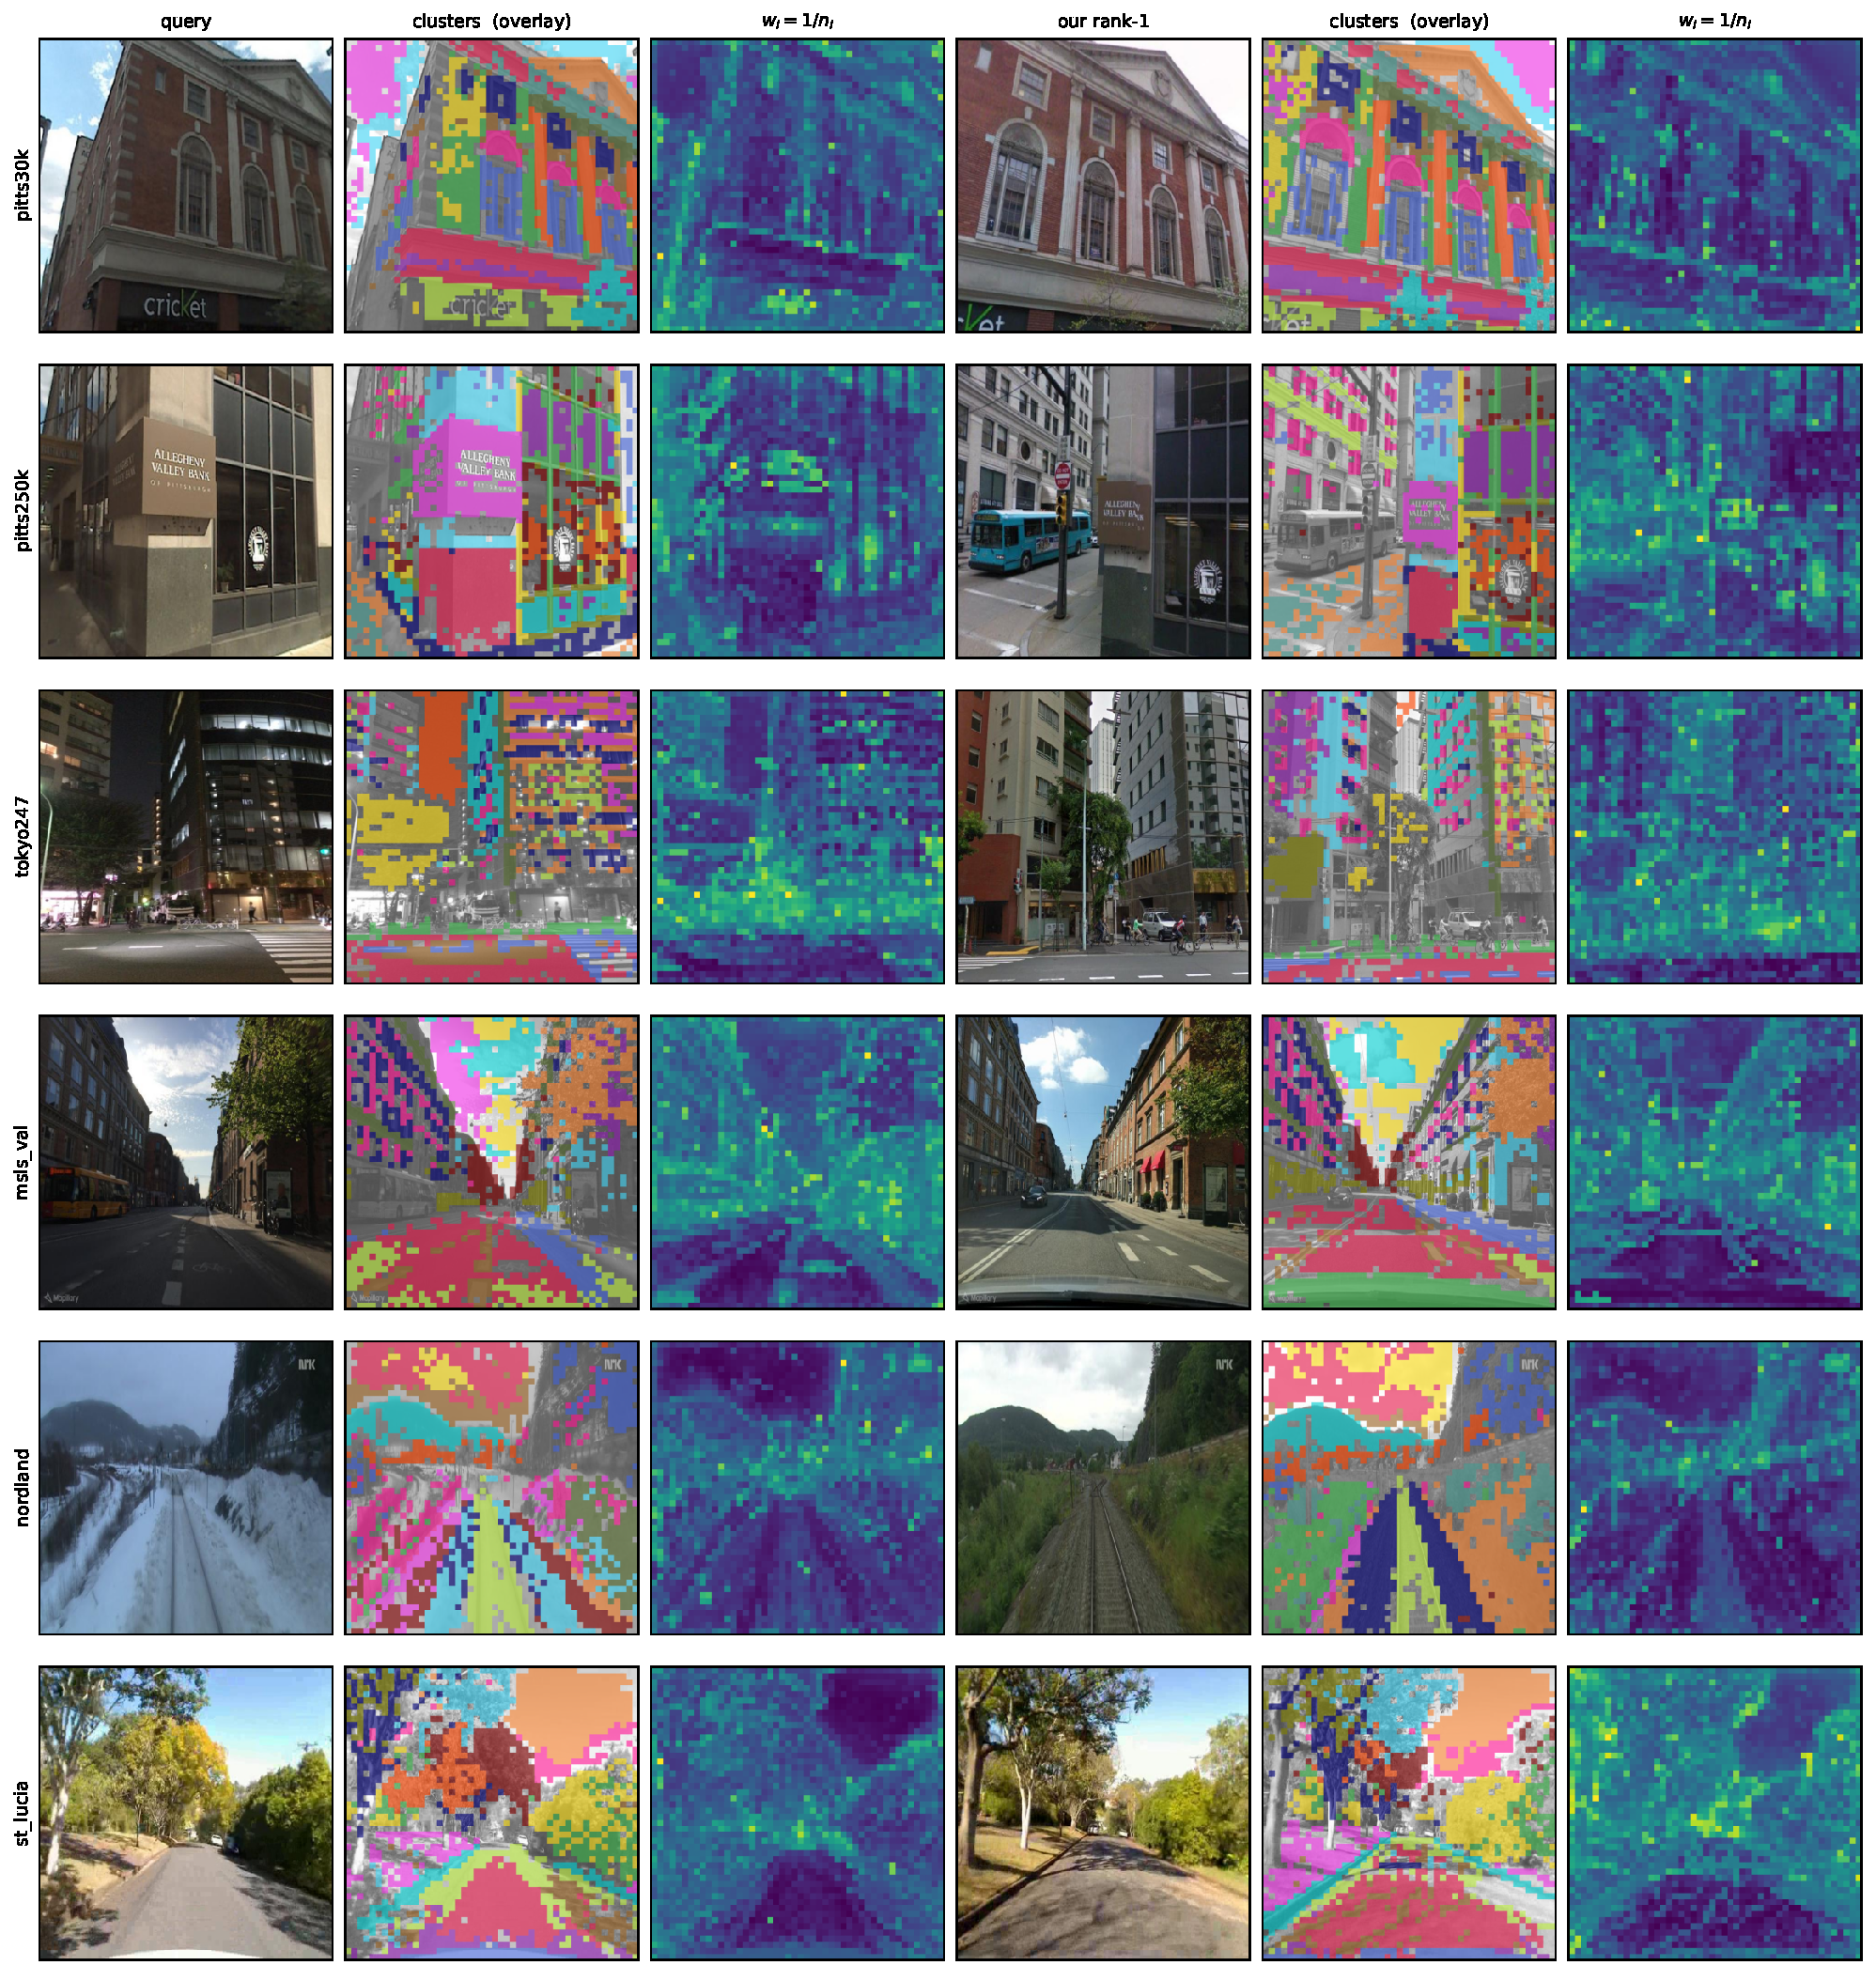
\includegraphics[width=\textwidth]{figures/all_clusters_1.pdf}
\caption{Near-duplicate blocks, benchmarks 1--6. Grey marks patches joining no block; the third and sixth columns show $w_i{=}1/n_i$ on a log scale over the full $2{,}304$ tokens.}
\label{fig:vis-c1}
\end{figure*}
\begin{figure*}[p]
\centering
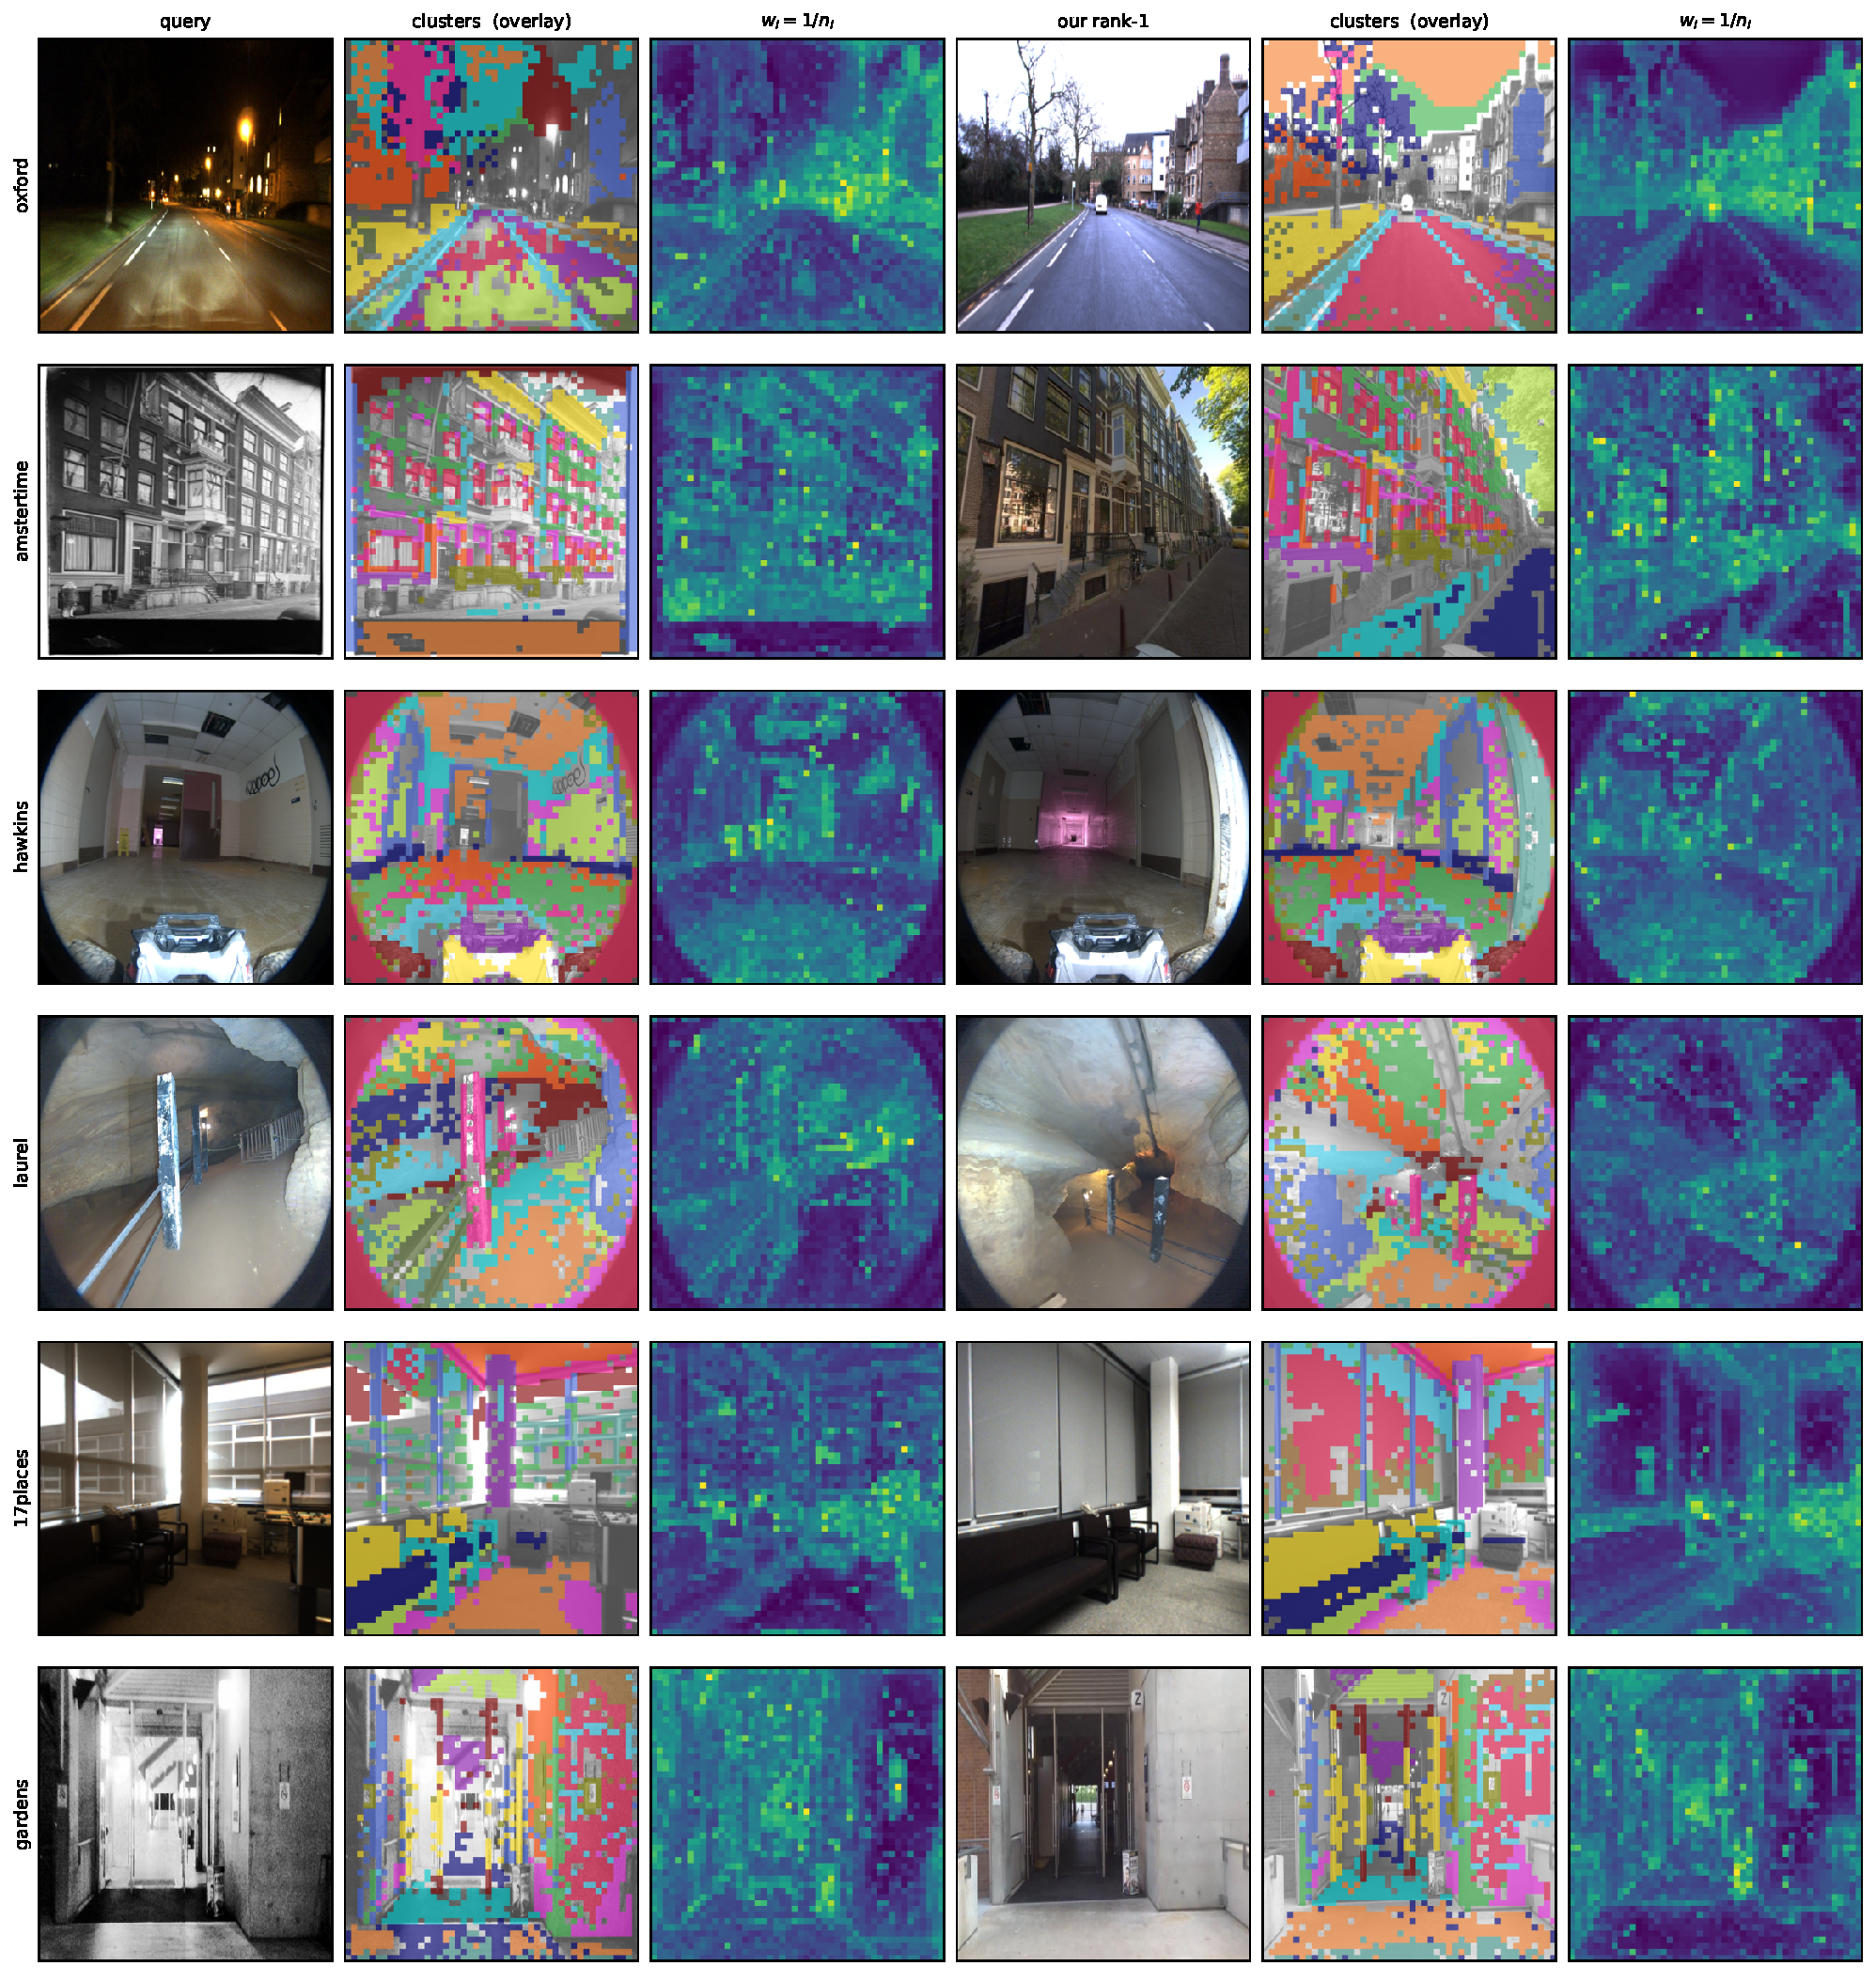
\includegraphics[width=\textwidth]{figures/all_clusters_2.pdf}
\caption{Near-duplicate blocks, benchmarks 7--12.}
\label{fig:vis-c2}
\end{figure*}
\begin{figure*}[p]
\centering
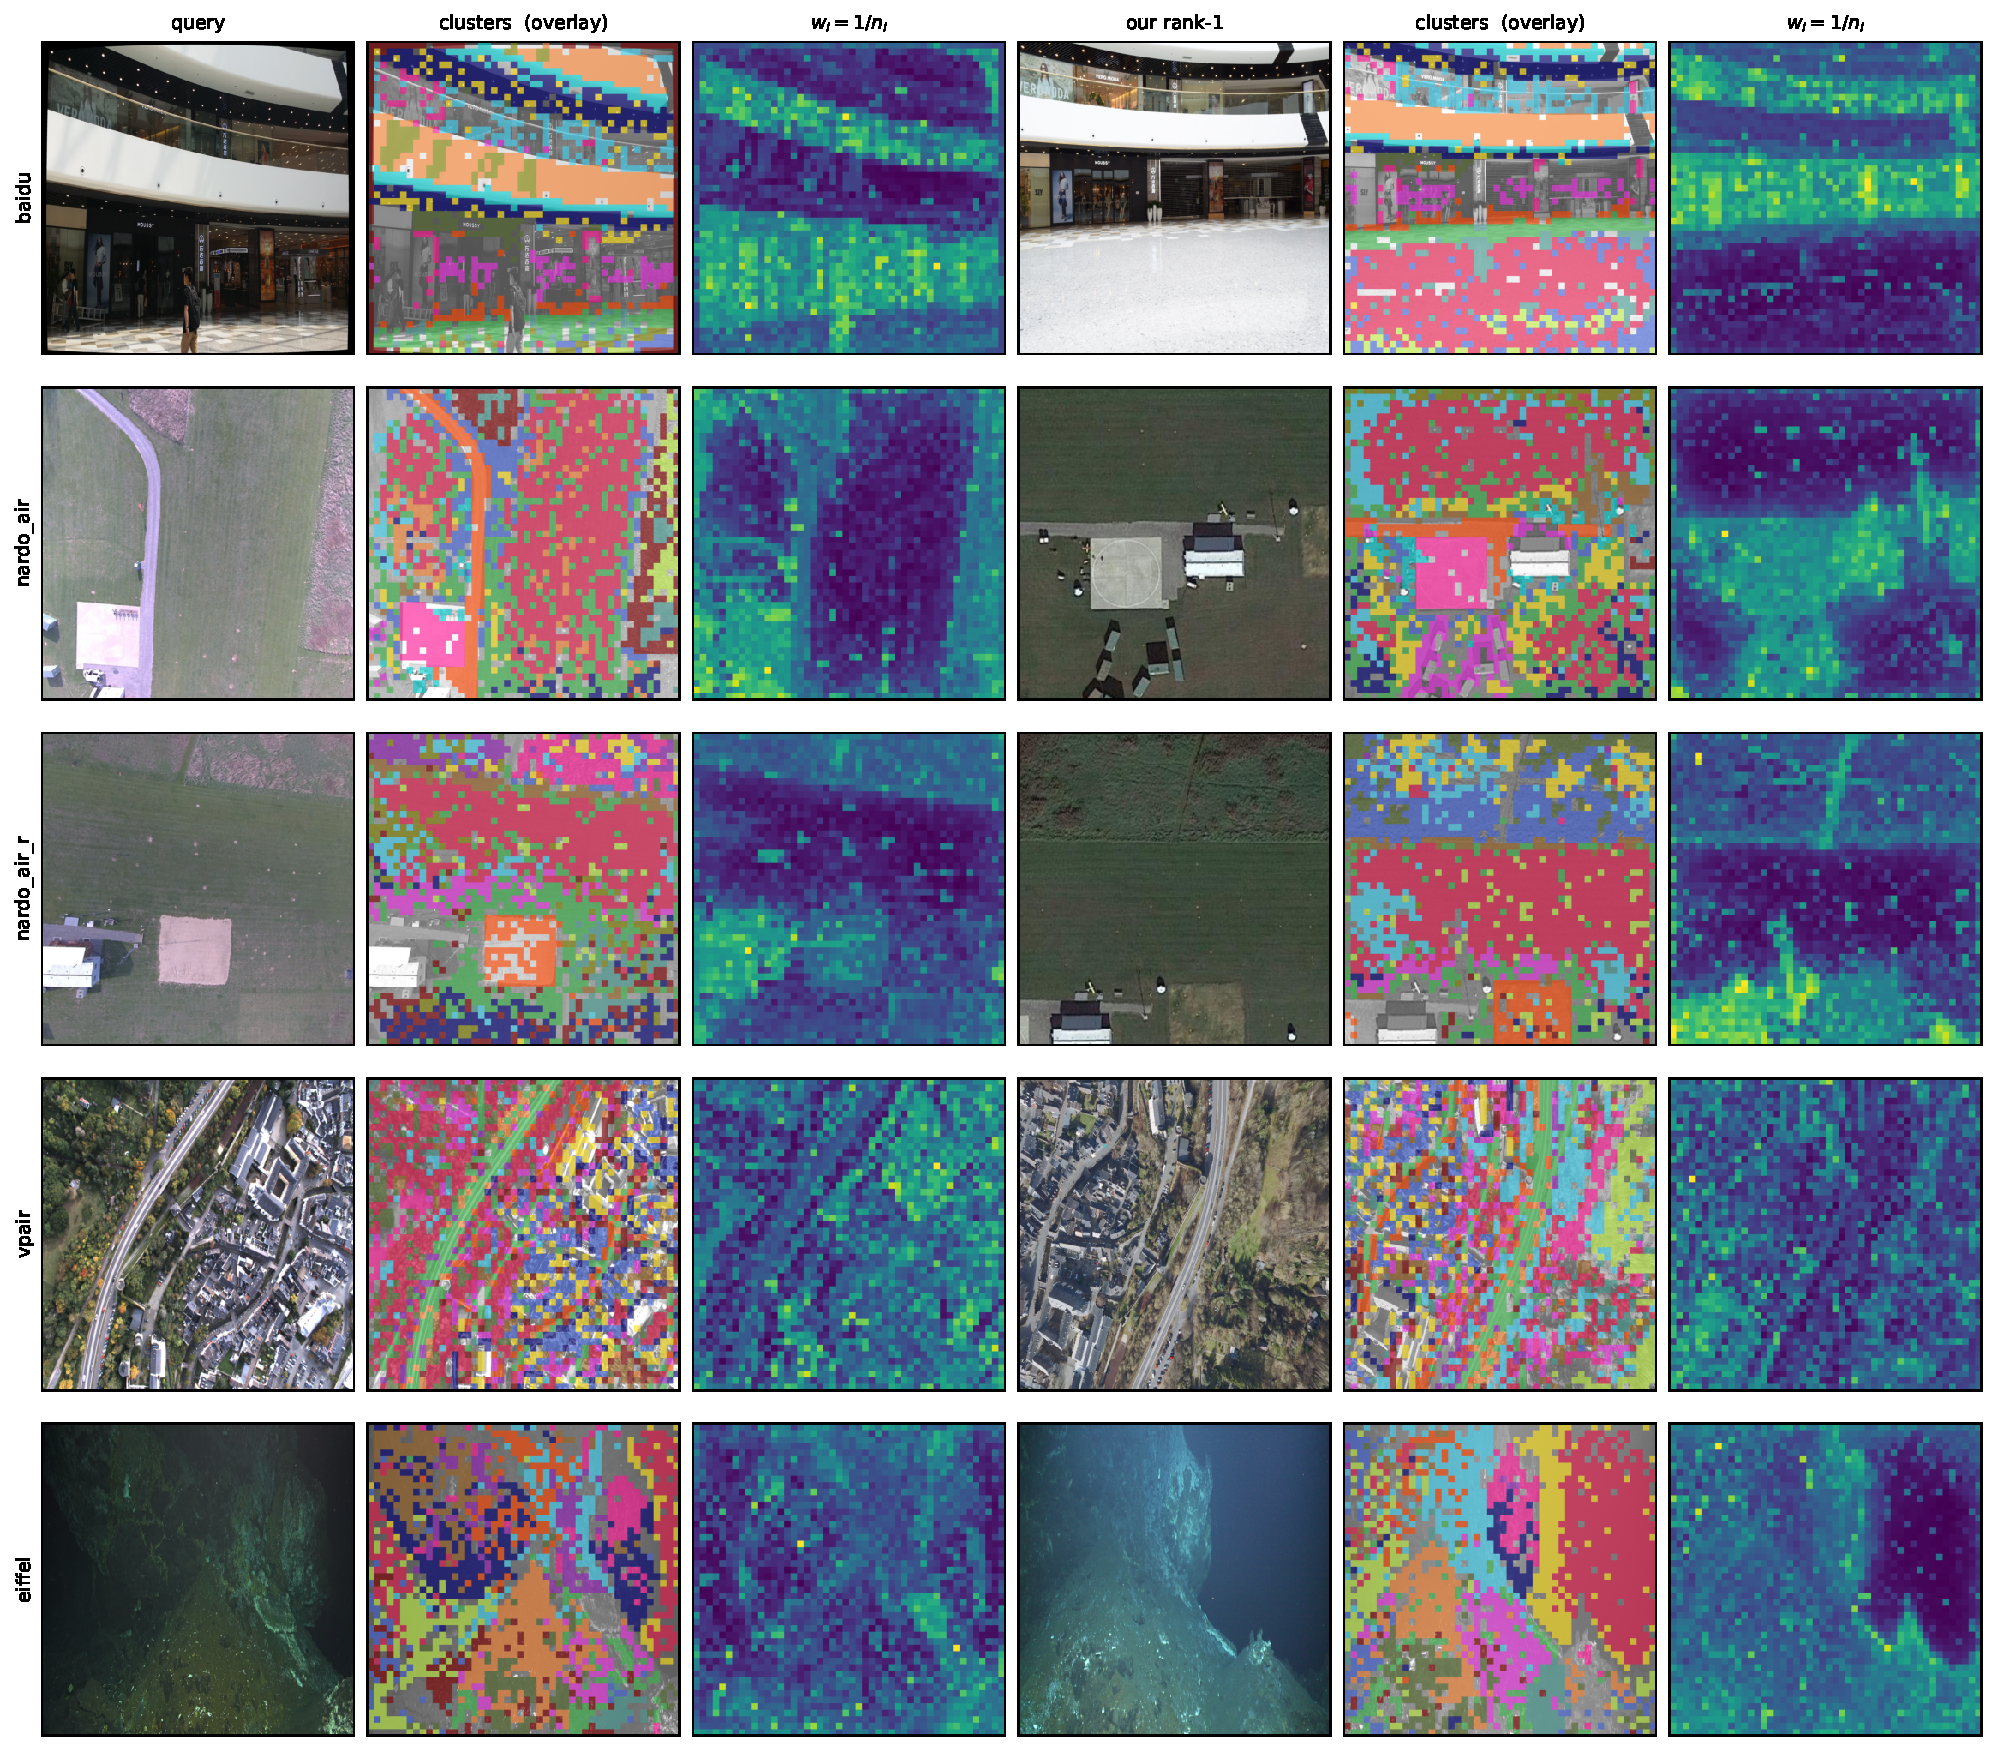
\includegraphics[width=\textwidth]{figures/all_clusters_3.pdf}
\caption{Near-duplicate blocks, benchmarks 13--17.}
\label{fig:vis-c3}
\end{figure*}

\section{The second-order descriptor}

\subsection{The coarse stage: factorial and reduction grid}
\label{sec:exp-stage1}
\label{sec:stage1abl}
\label{sec:compact}
\label{app:coarsegrid}
\begin{table}[t]
\caption{\textbf{Stage 1 alone on the nine environments.} R@1, single-stage global retrieval, every row our own run under one protocol at each method's native resolution. $^{\dagger}$reported after its own re-ranker; $^{o}$from our earlier operating point, as is the DINOv2-G row.}
\label{tab:coarse}
\begin{center}
{\scriptsize\setlength{\tabcolsep}{1.8pt}\renewcommand{\arraystretch}{0.86}%
\begin{tabular}{llccccccccc|c}
\toprule
& & Degr.\ & SubT & \multicolumn{3}{c}{Indoor} & \multicolumn{3}{c}{Aerial} & UW & \\
\cmidrule(lr){3-11}
Method   &   Backbone   &   Hawk   &   Laurel   &  17Pl &   Gard   &   Baidu   &   N-Air   &   N-AirR   &   VP-Air   & M-Atl &   mean \\
\midrule
\multicolumn{12}{l}{\emph{Trained / fine-tuned --- single-stage global descriptor}} \\
MegaLoc              &    DINOv2-B    &  37.3  &  55.4  &  64.8  &  95.5  &  \underline{79.4}  &  \textbf{85.9}  &  81.7  &  45.6  &  \textbf{40.6}  &  65.1\\
SAGE                 &    DINOv2-L    &  27.1  &  46.4  &  64.0  &  93.5  &  74.6  &  \textbf{85.9}  &  84.5  &  39.1  &  24.8  &  60.0\\
BoQ                  &    DINOv2-B    &  33.9  &  60.7  &  64.3  &  \underline{98.0}  &  77.4  &  62.0  &  91.5  &  29.5  &  35.6  &  61.4\\
CricaVPR             &    DINOv2-B    &  28.0  &  34.8  &  64.0  &  94.0  &  65.8  &  45.1  &  \textbf{100.0}  &  19.9  &  27.7  &  53.3\\
SALAD                &    DINOv2-B    &  38.1  &  46.4  &  64.3  &  96.5  &  69.9  &  53.5  &  94.4  &  24.0  &  15.8  &  55.9\\
CliqueMining         &    DINOv2-B    &  22.9  &  38.4  &  65.3  &  93.0  &  69.2  &  62.0  &  84.5  &  22.8  &  35.6  &  54.9\\
FoL$^{\dagger}$      & DINOv2-L       &  36.4  &  54.5  &  65.3  &  97.0  &  78.9  &  77.5  &  \underline{98.6}  &  46.7  &  25.7  &  64.5\\
EigenPlaces          &    R50         &  28.8  &  27.7  &  63.8  &  86.0  &  66.6  &  12.7  &  \textbf{100.0}  &  13.1  &  29.7  &  47.6\\
CosPlace             &    R50         &  33.9  &  25.9  &  63.3  &  84.5  &  47.1  &  0.0  &  76.1  &  10.4  &  32.7  &  41.5\\
SFRS                 &    VGG16       &  29.7  &  21.4  &  59.1  &  55.0  &  51.3  &  0.0  &  47.9  &  9.4  &  9.9  &  31.5\\
SelaVPR++$^{\dagger}$  &  DINOv2-L         &  21.2  &  35.7  &  65.0  &  95.5  &  73.6  &  81.7  &  87.3  &  42.7  &  27.7  &  58.9\\
Patch-NetVLAD        &    VGG16       &  39.0  &  59.8  &  63.1  &  74.5  &  66.8  &  63.4  &  71.8  &  16.0  &  23.8  &  53.1\\
R2Former$^{\dagger}$ & DeiT-S         &  17.8  &  30.4  &  63.8  &  84.0  &  74.7  &  26.8  &  83.1  &  15.0  &  22.8  &  46.5\\
VLAD-BuFF            &    DINOv2-B    &  37.3  &  33.9  &  64.5  &  96.5  &  76.4  &  57.8  &  88.7  &  33.3  &  27.7  &  57.4\\
SuperVLAD            &    DINOv2-B    &  37.3  &  51.8  &  64.8  &  95.5  &  70.3  &  14.1  &  88.7  &  23.8  &  13.9  &  51.1\\
SelaVPR$^{\dagger}$  & DINOv2-L       &  25.4  &  53.6  &  63.3  &  94.5  &  68.5  &  59.1  &  83.1  &  32.6  &  21.8  &  55.8\\
MixVPR               &    R50         &  26.3  &  32.1  &  63.8  &  92.0  &  68.4  &  39.4  &  78.9  &  12.9  &  24.8  &  48.7\\
NetVLAD              &    VGG16       &  38.1  &  42.9  &  63.8  &  66.0  &  57.8  &  9.9  &  39.4  &  14.7  &  26.7  &  39.9\\
\midrule
\multicolumn{12}{l}{\emph{Training-free --- frozen backbone, first-order pooling}} \\
GeM                  &    DINOv2-B    &  54.2  &  56.3  &  63.8  &  90.5  &  48.1  &  66.2  &  85.9  &  37.0  &  20.8  &  58.1\\
GeM                  &    DINOv2-L    &  55.9  &  56.3  &  63.8  &  92.5  &  46.4  &  \underline{80.3}  &  83.1  &  46.4  &  24.8  &  61.1\\
AnyLoc$^{p}$         &    DINOv2-G    &  \underline{65.2}  &  61.6  &  65.0  &  95.5  &  75.2  &  76.1  &  85.9  &  \underline{66.7}$^{d}$  &  34.6  &  \underline{69.5}\\
\midrule
\multicolumn{12}{l}{Ours \emph{--- training-free, second-order instance}} \\
Ours    &    DINOv2-B    &  58.5  &  60.7  &  63.6  &  94.0  &  71.7  &  47.9  &  84.5  &  43.0  &  35.6$^{o}$  &  62.2\\
Ours    &    DINOv2-L    &  \textbf{69.5}  &  50.9  &  64.0  &  96.0  &  73.8  &  36.6  &  84.5  &  49.5  &  \underline{36.6}$^{o}$  &  62.4\\
Ours    &    DINOv2-G    &  56.8  &  \underline{67.9}  &  65.0  &  96.5  &  76.7  &  74.7  &  95.8  &  48.2  &  35.6  &  68.6\\
Ours    &    DINOv3-L    &  59.3  &  \textbf{69.6}  &  64.3  &  95.0  &  78.2  &  42.3  &  87.3  &  56.0  &  31.7$^{o}$  &  64.9\\
Ours    &    DINOv3-7B    &  52.5  &  60.7  &  \underline{65.5}  &  95.5  &  77.2  &  74.7  &  95.8  &  \textbf{73.4}  &  34.7$^{o}$  &  \textbf{70.0}\\
\bottomrule
\end{tabular}%
}
\end{center}
\end{table}
\begin{table}[t]
\caption{\textbf{The instance-and-device factorial at a matched $1024$-d budget} (compressed before scoring). Uncompressed, the second order leads all six statistics; at this budget the orders trade domains, and the weight remains the largest device in both ($7.0$ and $18.7$ mean R@1).}
\label{tab:firstsecond}
\begin{center}
{\scriptsize\setlength{\tabcolsep}{2.2pt}%
\resizebox{\textwidth}{!}{%
\begin{tabular}{lccccccc|c}
\toprule
 & \multicolumn{7}{c}{per database} & \multicolumn{1}{c}{summary$^\dagger$} \\
\cmidrule(lr){2-8}\cmidrule(lr){9-9}
Configuration   &   Amst   &   SF$^\ast$   &   Pitts   &   VP-Air   &   MSLS   &   Nord   &   Tokyo   &   mean \\
    &  \tiny 1.2k &  \tiny 8.0k &  \tiny 10k &  \tiny 12.7k &  \tiny 18.9k &  \tiny 27.6k &  \tiny 76.0k & \\
\midrule \multicolumn{9}{l}{\emph{\textbf{R@1}} \ \ \scriptsize mean over the $6$ databases both orders share} \\
\multicolumn{9}{l}{\ \ First order (VLAD)} \\
\ \ \ none    &  26.16 &  52.67 &  74.94 &  44.09 &  34.46 &  10.89 &  68.89 &  40.54 \\
\ \ \ intra-norm    &  46.55 &  68.07 &  85.62 &  55.99 &  53.38 &  12.94 &  91.11 &  53.76 \\
\ \ \ power law    &  40.70 &  63.20 &  80.34 &  46.27 &  42.16 &  16.21 &  80.95 &  48.15 \\
\ \ \ intra-norm $+$ power law    &  47.77 &  68.85 &  85.18 &  52.73 &  52.03 &  15.92 &  88.89 &  53.75 \\
\ \ \ $w$    &  34.69 &  76.06 &  84.30 &  43.02 &  65.00 &  35.54 &  54.29 &  56.44 \\
\ \ \ $w$ $+$ intra-norm    &  46.95 &  63.94 &  85.14 &  52.18 &  51.22 &  15.13 &  88.57 &  52.43 \\
\ \ \ $w$ $+$ intra-norm $+$ power law    &  47.12 &  65.24 &  84.32 &  50.70 &  50.14 &  17.27 &  85.71 &  52.46 \\
\ \ \ \textbf{$w$ $+$ power law}    &  45.57 &  80.42 &  86.38 &  48.60 &  70.41 &  44.82 &  78.73 &  62.70 \\
\multicolumn{9}{l}{\ \ Second order (covariance)} \\
\ \ \ none    &  21.85 &  38.67 &  72.84 &  37.14 &  24.86 &  4.90 &    ---    &  33.38 \\
\ \ \ spectral $\alpha{=}\tfrac12$    &  34.12 &  54.68 &  80.55 &  40.06 &  36.89 &  10.93 &    ---    &  42.87 \\
\ \ \ power law    &  33.79 &  52.99 &  77.14 &  38.54 &  33.65 &  15.19 &    ---    &  41.88 \\
\ \ \ spectral $+$ power law    &  41.27 &  64.44 &  81.94 &  35.66 &  44.32 &  23.33 &    ---    &  48.49 \\
\ \ \ $w$    &  42.32 &  75.06 &  87.05 &  42.13 &  69.19 &  35.21 &    ---    &  58.49 \\
\ \ \ $w$ $+$ spectral    &  45.90 &  75.26 &  88.12 &  44.68 &  68.92 &  39.63 &    ---    &  60.42 \\
\ \ \ $w$ $+$ spectral $+$ power law    &  46.71 &  73.61 &  88.04 &  38.06 &  67.84 &  51.19 &    ---    &  60.91 \\
\ \ \ \textbf{$w$ $+$ power law}    &  45.49 &  74.46 &  87.40 &  43.83 &  68.11 &  51.39 &    ---    &  61.78 \\
\midrule \multicolumn{9}{l}{\emph{\textbf{R@100}} \ \ \scriptsize mean over the $6$ databases both orders share} \\
\multicolumn{9}{l}{\ \ First order (VLAD)} \\
\ \ \ none    &  79.45 &  83.87 &  95.25 &  79.34 &  62.84 &  39.58 &  96.19 &  73.39 \\
\ \ \ intra-norm    &  93.58 &  95.99 &  99.16 &  90.28 &  86.89 &  51.10 &  98.73 &  86.17 \\
\ \ \ power law    &  91.71 &  93.80 &  97.29 &  83.07 &  78.24 &  51.98 &  98.73 &  82.68 \\
\ \ \ intra-norm $+$ power law    &  94.48 &  96.42 &  99.11 &  88.40 &  85.54 &  54.32 &  98.41 &  86.38 \\
\ \ \ $w$    &  90.33 &  97.80 &  98.93 &  90.84 &  92.57 &  81.13 &  92.06 &  91.93 \\
\ \ \ $w$ $+$ intra-norm    &  93.99 &  95.59 &  99.18 &  92.76 &  87.57 &  53.75 &  98.10 &  87.14 \\
\ \ \ $w$ $+$ intra-norm $+$ power law    &  94.23 &  96.22 &  98.99 &  90.24 &  85.81 &  55.19 &  98.10 &  86.78 \\
\ \ \ \textbf{$w$ $+$ power law}    &  94.48 &  98.18 &  99.16 &  89.06 &  95.14 &  82.27 &  97.14 &  93.05 \\
\multicolumn{9}{l}{\ \ Second order (covariance)} \\
\ \ \ none    &  71.32 &  69.26 &  93.79 &  71.91 &  53.92 &  24.28 &    ---    &  64.08 \\
\ \ \ spectral $\alpha{=}\tfrac12$    &  87.00 &  87.71 &  96.96 &  72.84 &  71.62 &  40.56 &    ---    &  76.11 \\
\ \ \ power law    &  88.87 &  87.86 &  96.13 &  74.32 &  67.70 &  47.43 &    ---    &  77.05 \\
\ \ \ spectral $+$ power law    &  91.96 &  94.23 &  97.48 &  68.96 &  77.84 &  59.82 &    ---    &  81.72 \\
\ \ \ $w$    &  92.36 &  96.73 &  99.19 &  84.29 &  94.32 &  77.41 &    ---    &  90.72 \\
\ \ \ $w$ $+$ spectral    &  93.34 &  96.78 &  99.33 &  82.22 &  93.65 &  77.82 &    ---    &  90.52 \\
\ \ \ $w$ $+$ spectral $+$ power law    &  93.99 &  96.72 &  99.35 &  76.09 &  93.24 &  84.06 &    ---    &  90.58 \\
\ \ \ \textbf{$w$ $+$ power law}    &  93.74 &  97.03 &  99.24 &  85.03 &  94.19 &  85.63 &    ---    &  92.48 \\
\midrule \multicolumn{9}{l}{\emph{\textbf{R@1000}} \ \ \scriptsize mean over the $4$ databases both orders share; AmsterTime and SF-XL val are shown but excluded from the summary, where a top-$1000$ list is $81\%$ and $12.5\%$ of the database} \\
\multicolumn{9}{l}{\ \ First order (VLAD)} \\
\ \ \ none    &  99.43 &  98.70 &  99.87 &  96.05 &  87.97 &  76.66 &  \textbf{100.00} &  90.14 \\
\ \ \ intra-norm    &  \textbf{100.00} &  99.84 &  \textbf{100.00} &  \textbf{99.78} &  97.70 &  81.03 &  \textbf{100.00} &  94.63 \\
\ \ \ power law    &  99.84 &  99.84 &  \textbf{100.00} &  98.45 &  96.49 &  83.37 &  \underline{99.68} &  94.58 \\
\ \ \ intra-norm $+$ power law    &  \textbf{100.00} &  \textbf{99.91} &  \textbf{100.00} &  \textbf{99.78} &  98.11 &  83.06 &  \underline{99.68} &  95.24 \\
\ \ \ $w$    &  99.84 &  99.87 &  \textbf{100.00} &  99.70 &  98.11 &  \underline{97.19} &  99.05 &  98.75 \\
\ \ \ $w$ $+$ intra-norm    &  \textbf{100.00} &  99.80 &  \textbf{100.00} &  \underline{99.74} &  98.11 &  81.53 &  \underline{99.68} &  94.84 \\
\ \ \ $w$ $+$ intra-norm $+$ power law    &  \textbf{100.00} &  99.86 &  \textbf{100.00} &  \underline{99.74} &  98.11 &  83.51 &  99.05 &  95.34 \\
\ \ \ \textbf{$w$ $+$ power law}    &  \textbf{100.00} &  \underline{99.90} &  \textbf{100.00} &  \textbf{99.78} &  \textbf{99.05} &  97.03 &  \underline{99.68} &  \underline{98.97} \\
\multicolumn{9}{l}{\ \ Second order (covariance)} \\
\ \ \ none    &  99.76 &  90.81 &  \underline{99.88} &  94.09 &  77.70 &  60.02 &    ---    &  82.92 \\
\ \ \ spectral $\alpha{=}\tfrac12$    &  \underline{99.92} &  98.91 &  \textbf{100.00} &  95.45 &  90.00 &  75.87 &    ---    &  90.33 \\
\ \ \ power law    &  \underline{99.92} &  99.36 &  \textbf{100.00} &  93.31 &  90.54 &  82.27 &    ---    &  91.53 \\
\ \ \ spectral $+$ power law    &  \textbf{100.00} &  99.76 &  \textbf{100.00} &  94.38 &  96.22 &  86.25 &    ---    &  94.21 \\
\ \ \ $w$    &  \textbf{100.00} &  99.85 &  \textbf{100.00} &  99.19 &  98.24 &  94.32 &    ---    &  97.94 \\
\ \ \ $w$ $+$ spectral    &  \textbf{100.00} &  99.89 &  \textbf{100.00} &  98.97 &  \underline{98.38} &  94.30 &    ---    &  97.91 \\
\ \ \ $w$ $+$ spectral $+$ power law    &  \textbf{100.00} &  99.87 &  \textbf{100.00} &  99.26 &  98.24 &  96.84 &    ---    &  98.59 \\
\ \ \ \textbf{$w$ $+$ power law}    &  \textbf{100.00} &  99.84 &  \textbf{100.00} &  99.67 &  98.24 &  \textbf{98.12} &    ---    &  \textbf{99.01} \\
\bottomrule
\end{tabular}%
}%
}
\end{center}
\end{table}
\begin{table}[t]
\caption{\textbf{Token pruning $\times$ whitened compression, single-stage coarse retrieval} (R@1; five test benchmarks and their mean). Both orders, both backbones, one protocol; keep-$N$ selects by $w_i$ computed on the full token set. $^\dagger$AmsterTime rank-caps the WPCA below $2{,}048$-d; its $1{,}024$-d value shown. R@1000 never falls below $98.4$ (7B) / $96.3$ (L) anywhere in the grid.}
\label{tab:prunecomp}
\begin{center}
\scriptsize
\setlength{\tabcolsep}{3.4pt}
\renewcommand{\arraystretch}{1.02}
\resizebox{\textwidth}{!}{%
\begin{tabular}{lll rrrrr r rrrrr r}
\toprule
& & & \multicolumn{6}{c}{DINOv3-7B} & \multicolumn{6}{c}{DINOv3-L} \\
\cmidrule(lr){4-9}\cmidrule(lr){10-15}
Order   &   keep   &   compression   &   Pitts   &   MSLS   &   Nord   &   Tokyo   &   Amst   &   mean   &   Pitts   &   MSLS   &   Nord   &   Tokyo   &   Amst   &   mean \\
\midrule
2nd   &   full    &   raw              &  88.51 &  70.95 &  63.98 &  93.02 &  51.58 &  73.61 &  88.97 &  69.73 &  43.82 &  91.75 &  44.27 &  67.71\\
       &             &    WPCA-1024         &  89.61 &  83.78 &  60.14 &  93.65 &  67.67 &  78.97 &  89.67 &  82.57 &  37.47 &  90.48 &  61.49 &  72.34\\
       &             &    WPCA-2048         &  89.80 &  86.49 &  62.18 &  95.87 &  67.67$^\dagger$ &  80.40 &  89.57 &  84.19 &  42.19 &  92.38 &  61.49$^\dagger$ &  73.96\\
\addlinespace[2pt]
2nd   &   1024    &   raw              &  89.22 &  74.32 &  69.33 &  92.06 &  48.09 &  74.60 &  89.10 &  73.65 &  44.31 &  87.30 &  40.29 &  66.93\\
       &             &    WPCA-1024         &  90.45 &  84.86 &  70.78 &  92.70 &  66.04 &  80.97 &  89.99 &  84.05 &  43.98 &  86.67 &  59.55 &  72.85\\
       &             &    \textbf{WPCA-2048}    &  91.02 &  86.89 &  75.09 &  94.92 &  66.04$^\dagger$ &  82.79 &  90.64 &  84.19 &  49.75 &  90.79 &  59.55$^\dagger$ &  74.98\\
\addlinespace[2pt]
2nd   &   512     &   raw              &  87.71 &  74.05 &  71.17 &  85.40 &  40.62 &  71.79 &  87.29 &  72.43 &  43.58 &  81.90 &  33.23 &  63.69\\
       &             &    WPCA-1024         &  90.40 &  84.19 &  74.26 &  89.52 &  60.52 &  79.78 &  89.50 &  84.05 &  48.66 &  83.49 &  51.18 &  71.38\\
       &             &    WPCA-2048         &  91.07 &  86.76 &  78.06 &  93.33 &  60.52$^\dagger$ &  81.95 &  90.60 &  82.97 &  53.81 &  89.21 &  51.18$^\dagger$ &  73.55\\
\midrule
1st   &   full    &   raw              &  86.52 &  71.22 &  67.41 &  92.70 &  52.40 &  74.05 &  86.84 &  67.16 &  40.27 &  90.48 &  45.90 &  66.13\\
       &             &    WPCA-1024         &  87.32 &  84.05 &  56.07 &  94.29 &  62.47 &  76.84 &  87.24 &  77.70 &  30.26 &  92.70 &  55.89 &  68.76\\
       &             &    WPCA-2048         &  87.21 &  83.24 &  54.37 &  95.56 &  62.47$^\dagger$ &  76.57 &  86.75 &  79.59 &  30.07 &  91.11 &  55.89$^\dagger$ &  68.68\\
\addlinespace[2pt]
1st   &   1024    &   raw              &  87.62 &  77.03 &  79.56 &  89.84 &  51.26 &  77.06 &  87.28 &  72.30 &  49.61 &  87.30 &  44.11 &  68.12\\
       &             &    WPCA-1024         &  88.47 &  85.00 &  61.48 &  92.06 &  60.03 &  77.41 &  88.15 &  81.62 &  34.48 &  88.89 &  53.05 &  69.24\\
       &             &    WPCA-2048         &  88.98 &  85.00 &  59.55 &  95.56 &  60.03$^\dagger$ &  77.82 &  88.50 &  80.68 &  35.13 &  89.52 &  53.05$^\dagger$ &  69.38\\
\addlinespace[2pt]
1st   &   512     &   raw              &  85.52 &  77.70 &  79.54 &  81.59 &  44.60 &  73.79 &  86.15 &  71.89 &  49.62 &  80.95 &  37.69 &  65.26\\
       &             &    WPCA-1024         &  87.57 &  84.32 &  61.93 &  85.08 &  51.42 &  74.06 &  86.83 &  79.46 &  35.88 &  79.37 &  43.54 &  65.02\\
       &             &    WPCA-2048         &  87.60 &  83.92 &  58.96 &  87.94 &  51.42$^\dagger$ &  73.97 &  87.50 &  79.73 &  36.78 &  81.59 &  43.54$^\dagger$ &  65.83\\
\bottomrule
\end{tabular}}
\end{center}
\end{table}

\subsection{What the weight does to the descriptor}
\label{app:patchvis-main}
\begin{figure}[H]
\centering
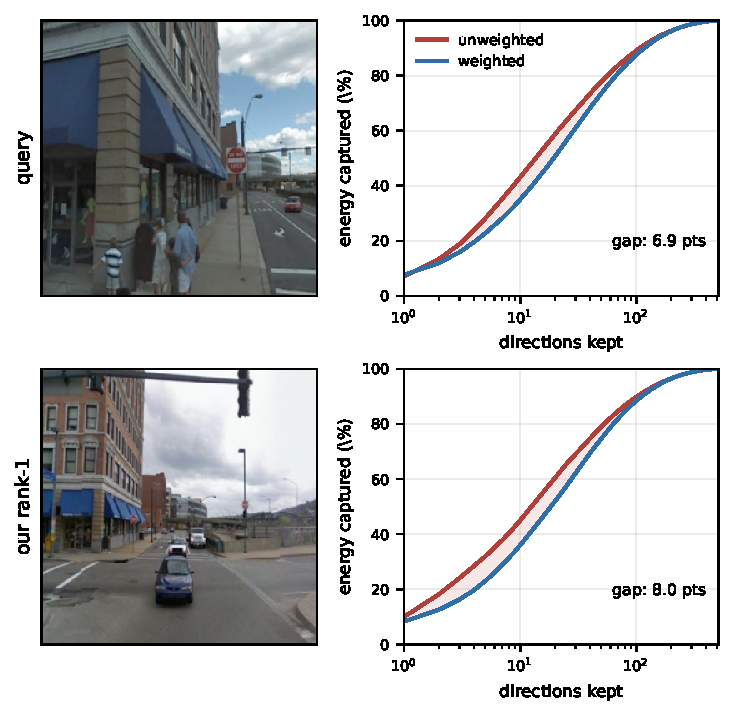
\includegraphics[width=0.50\textwidth]{figures/patch_cov.pdf}
\caption{\textbf{What the weight does to the descriptor.} One query and the database image our first stage retrieves for it. The right column reads $F^{\top}F$ and $G_C{=}F^{\top}WF$ as a distribution of the image's energy over directions: keeping the $k$ strongest directions captures the plotted share of the total, so a curve that rises early is one where a few directions carry the image. An element covering much of the frame arrives as many near-identical patches pointing the same way and concentrates the unweighted moment; the weight spreads it back, by $6.9$ and $8.0$ points averaged over the first $32$ directions.}
\label{fig:patchcov}
\end{figure}

\section{\textsc{MaxSim} re-ranking}

\subsection{Token budget against re-ranking operator}
\label{app:s2grid}
\begin{table}[h]
\caption{\textbf{Seven re-ranking operators $\times$ two token budgets}, mean R@1 over the nine environment sets of Table~\ref{tab:ood}. The coarse stage is the deployed one throughout; only the second stage changes. \textsc{selfw\_conf} is \eqref{eq:stage2}, the operator we adopt.}
\label{tab:s2grid}
\begin{center}
{\footnotesize\setlength{\tabcolsep}{3pt}%
\begin{tabular}{llccccccc}
\toprule
Backbone & tokens & base & \textsc{selfw} & \textsc{conf} & \textsc{selfw\_conf} & \textsc{mnn} & \textsc{mnn\_selfw} & comb. \\
\midrule
DINOv3-L  & keep-$1024$ & \textbf{74.85} & 74.07 & 73.89 & 73.56 & 71.10 & 70.74 & 70.50 \\
DINOv3-L  & all $2{,}304$ & 72.56 & 74.13 & 72.43 & \textbf{75.42} & 70.15 & 71.48 & 70.81 \\
\addlinespace[2pt]
DINOv3-7B & keep-$1024$ & 75.27 & 75.41 & 74.50 & \textbf{76.30} & 74.34 & 70.72 & 70.56 \\
DINOv3-7B & all $2{,}304$ & 71.68 & 74.90 & 69.04 & \textbf{76.57} & 70.46 & 72.10 & 71.63 \\
\bottomrule
\end{tabular}%
}
\end{center}
\end{table}

\subsection{Against \textsc{EffoVPR}'s criterion at a matched stage 1}
\label{app:effo-matched}
\begin{table}[t]
\caption{\textbf{Scoring rules at a matched stage 1} (Pitts30k, R@1; shortlist and features identical). \emph{lift} is over the class-token retrieval that produced the shortlist. $T_1$ is \textsc{EffoVPR}'s attention threshold, reported at the keypoint budget it induces.}
\label{tab:effo-matched}
\begin{center}
{\small
\begin{tabular}{lcc}
\toprule
Stage 2 & R@1 & lift \\
\midrule
none (class-token retrieval) & 77.93 & --- \\
\midrule
\multicolumn{3}{l}{\emph{Selection by attention} (\textsc{EffoVPR})} \\
keep all, mutual NN & 87.82 & $+9.89$ \\
$T_1$ at $512$ keypoints & \underline{88.70} & $+10.77$ \\
$T_1$ at $256$ & 86.66 & $+8.73$ \\
$T_1$ at $130$ & 82.51 & $+4.58$ \\
$T_1$ at $65$ & 77.93 & $+0.00$ \\
\midrule
\multicolumn{3}{l}{\emph{Weighting by self-similarity} (ours)} \\
\textsc{MaxSim}, unweighted & 86.53 & $+8.60$ \\
\textsc{selfw} & 91.31 & $+13.38$ \\
\textsc{selfw\_conf} & 91.24 & $+13.31$ \\
\textsc{mnn\_selfw65} & \textbf{91.58} & $+13.64$ \\
\bottomrule
\end{tabular}}
\end{center}
\end{table}
\begin{table}[t]
\caption{\textbf{Which patches to keep} (Pitts30k, R@1; survivors re-weighted by $w$ in every column). Symmetric keeps $N$ tokens in the query and in the database image; database-only keeps all query tokens. Keep-all reads $91.31$.}
\label{tab:keepn}
\begin{center}
{\small
\begin{tabular}{llccc}
\toprule
 & keep-$N$ & self-similarity & attention & random \\
\midrule
\multirow{4}{*}{symmetric}
 & $256$ ($5\times$)  & \textbf{91.08} & 87.62 & 87.49 \\
 & $128$ ($10\times$) & \textbf{88.44} & 82.91 & 81.92 \\
 & $64$ ($20\times$)  & \textbf{82.75} & 76.88 & 70.79 \\
 & $32$ ($40\times$)  & \textbf{72.17} & 70.42 & 55.59 \\
\midrule
\multirow{4}{*}{database only}
 & $256$ & 89.08 & 80.97 & \textbf{89.80} \\
 & $128$ & 82.72 & 69.53 & \textbf{87.65} \\
 & $64$  & 71.41 & 56.31 & \textbf{84.86} \\
 & $32$  & 58.98 & 45.70 & \textbf{80.05} \\
\bottomrule
\end{tabular}}
\end{center}
\end{table}

\subsection{\textsc{MaxSim} matches on every benchmark}
\label{app:patchvis-maxsim}
\begin{figure*}[p]
\centering
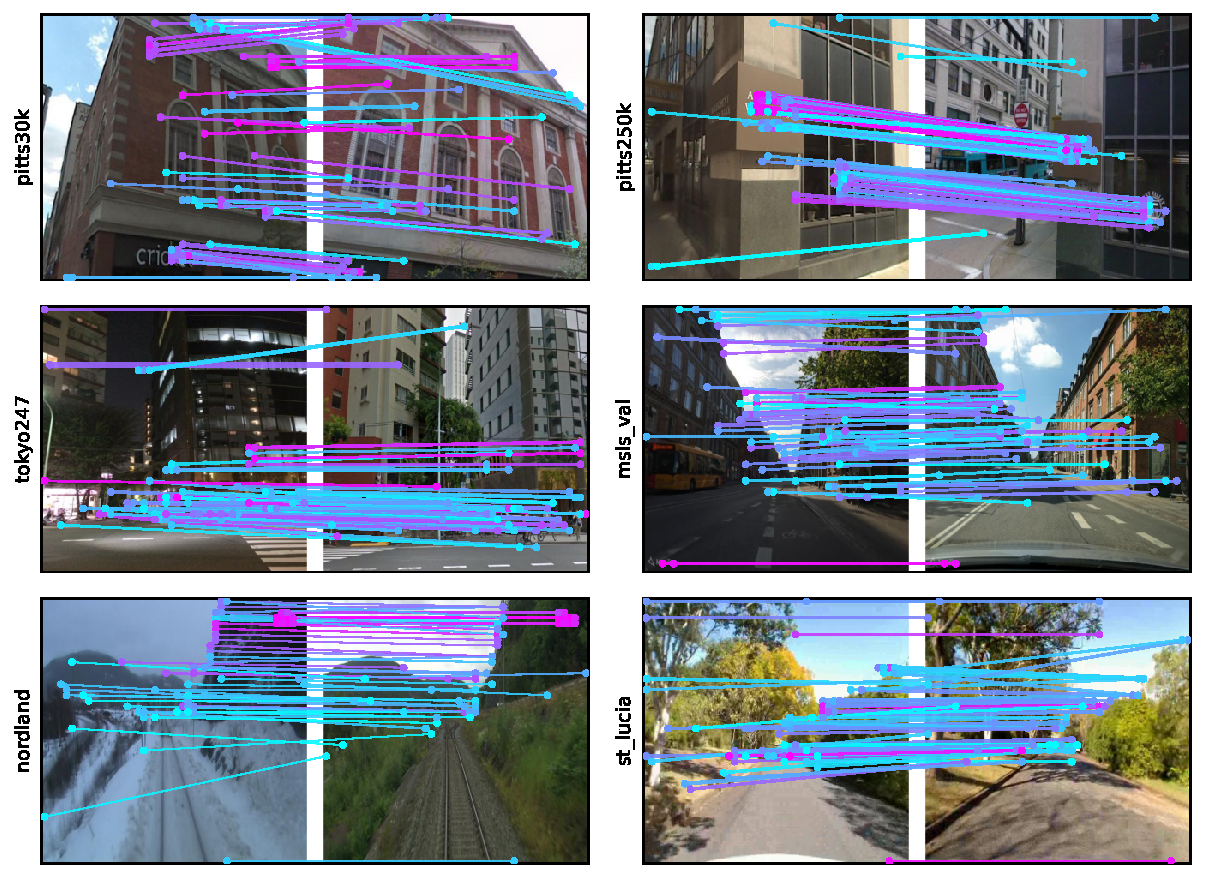
\includegraphics[width=\textwidth]{figures/all_maxsim_1.pdf}
\caption{\textsc{MaxSim} matches, benchmarks 1--6. Each line joins a query patch to its \textsc{MaxSim} partner in the retrieved image, drawn for the sixty largest contributions among the patches clearing the gate $\theta{=}0.65$ of \eqref{eq:stage2}; line colour is the row maximum $m_i$ and line width is that patch's contribution $c_i{=}w_i m_i$.}
\label{fig:vis-m1}
\end{figure*}
\begin{figure*}[p]
\centering
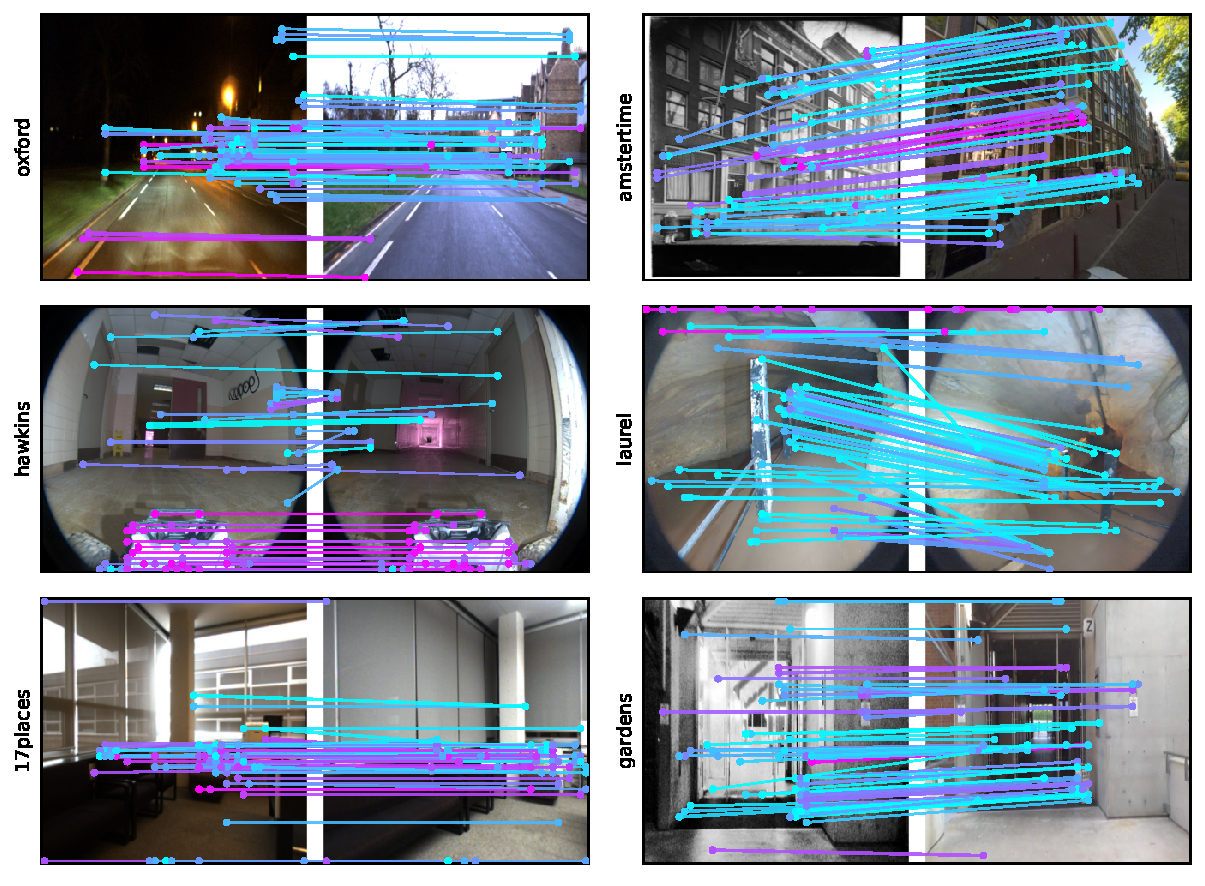
\includegraphics[width=\textwidth]{figures/all_maxsim_2.pdf}
\caption{\textsc{MaxSim} matches, benchmarks 7--12.}
\label{fig:vis-m2}
\end{figure*}
\begin{figure*}[p]
\centering
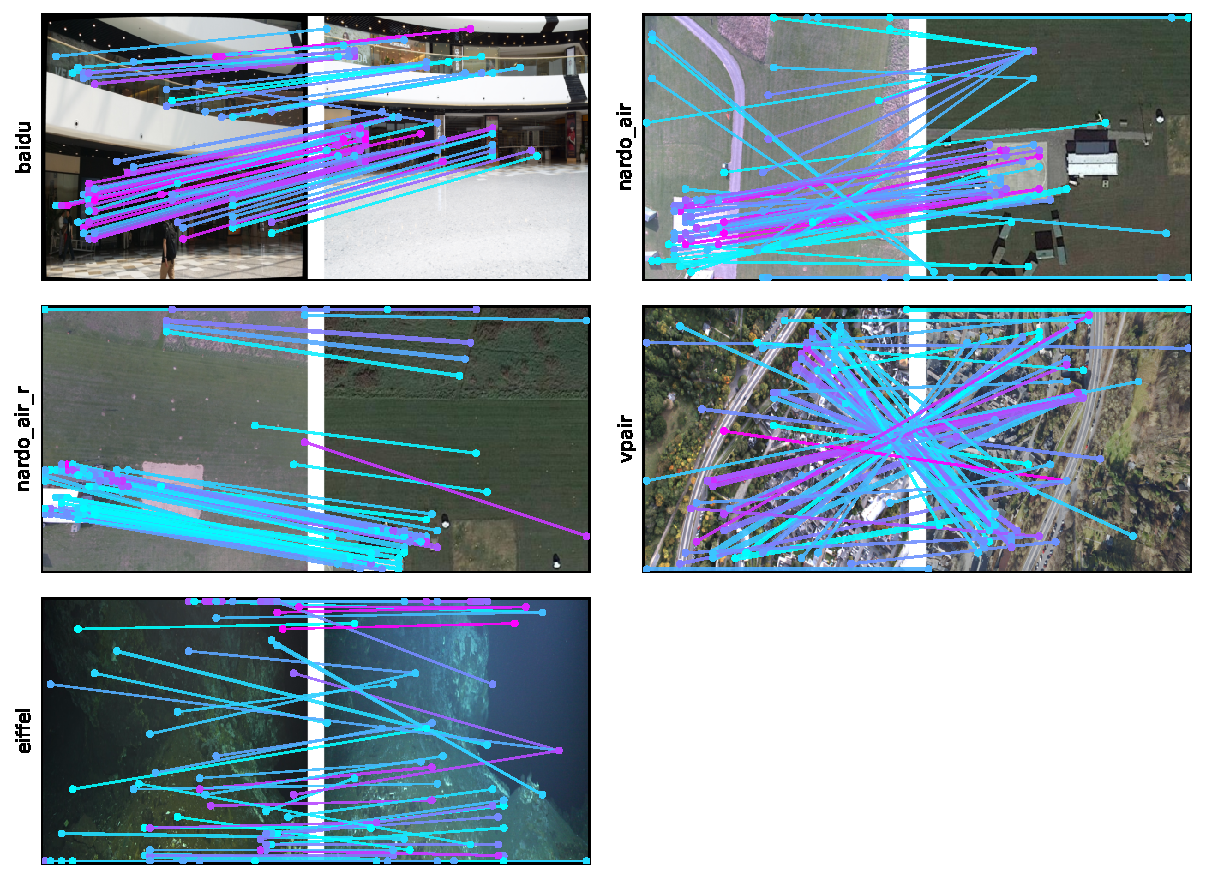
\includegraphics[width=\textwidth]{figures/all_maxsim_3.pdf}
\caption{\textsc{MaxSim} matches, benchmarks 13--17.}
\label{fig:vis-m3}
\end{figure*}

\section{Protocols and constants}

\subsection{Evaluation protocol}
\label{app:protocol}
\begin{table}[t]
\caption{\textbf{Evaluation protocol, per benchmark.} Every method here---ours and every baseline---is run through this protocol: same splits, ground truth and database. We do not quote each paper's own number, since those use different ground-truth radii and query subsets.}
\label{tab:protocol}
\begin{center}
{\scriptsize\setlength{\tabcolsep}{3.2pt}%
\resizebox{\textwidth}{!}{%
\begin{tabular}{lrrrll}
\toprule
Dataset & Database & Queries & Positives & Ground truth & Notes \\
\midrule
\multicolumn{6}{l}{\emph{Urban / standard benchmarks}} \\
\midrule
Pitts30k & 10{,}000 & 6{,}816 & 142.1 & UTM $\le 25$\,m & NetVLAD's official pitts30k\_test.mat split \\
Pitts250k & 83{,}952 & 8{,}280 & 153.6 & UTM $\le 25$\,m & same convention, different .mat \\
Tokyo 24/7 & 75{,}984 & 315 & 118.3 & filename UTM $\le 25$\,m & the official \textbf{315} subset, not the 1125 one \\
MSLS-val & 18{,}871 & 740 & 10.8 & filename UTM $\le 25$\,m, distance only (no heading) & the \textbf{740} subset of \citet{patchnetvlad}; \citet{effovpr} report the 11k variant \\
Nordland & 27{,}592 & 27{,}592 & 21.0 & $\pm 10$ frames (\textbf{lenient}) & papers using $\pm 1$ frame report markedly lower numbers \\
St Lucia & 1{,}549 & 1{,}464 & 14.9 & filename UTM $\le 25$\,m & gmberton format \\
Oxford RobotCar & 191 & 191 & 14.2 & the .mat's own posDistThr $=16$\,m & the small vehicular split used by \citet{anyloc} \\
AmsterTime & 1{,}231 & 1{,}231 & 1.0 & old\_X$\leftrightarrow$new\_X, one positive & historical against present-day photographs \\
\midrule
\multicolumn{6}{l}{\emph{SF-XL (one imagery set: a design split and four test splits)}} \\
\midrule
SF-XL val$^\ast$ & 8{,}015 & 7{,}983 & 9.3 & UTM $\le 25$\,m & \textbf{design split}; appears in no main table \\
SF-XL test v1 & 2{,}805{,}840 & 1{,}000 & 124.2 & UTM $\le 25$\,m & the four test splits share one $2.8$M database \\
SF-XL test v2 & 2{,}805{,}840 & 598 & 188.3 & UTM $\le 25$\,m & not yet re-run for the baselines (\S\ref{sec:setup}) \\
SF-XL test night & 2{,}805{,}840 & 466 & 114.1 & UTM $\le 25$\,m &  \\
SF-XL test occl. & 2{,}805{,}840 & 76 & 151.9 & UTM $\le 25$\,m & $74$ queries have a positive \\
\midrule
\multicolumn{6}{l}{\emph{Beyond street view (AnyLoc suite)}} \\
\midrule
VP-Air \emph{(aerial)} & 12{,}706 & 2{,}706 & 7.0 & provided correspondences & AnyLoc convention: database $=$ references $+$ $10{,}000$ distractors \\
Nardo-Air \emph{(aerial)} & 102 & 71 & 6.1 & gt\_matches.csv, distance $\le 60$\,m &  \\
Nardo-Air R \emph{(aerial)} & 102 & 71 & 6.1 & as above & reference images rotated $90^\circ$ \\
Hawkins \emph{(subterranean)} & 127 & 118 & 10.6 & 2-D pose $\le 8$\,m & long corridor \\
Laurel Caverns \emph{(subterranean)} & 141 & 112 & 23.8 & 2-D pose $\le 8$\,m &  \\
17 Places \emph{(indoor)} & 406 & 406 & 10.9 & official ground\_truth\_new.npy &  \\
Baidu Mall \emph{(indoor)} & 689 & 2{,}292 & 35.1 & 2-D camera pose $\le 10$\,m & $2{,}248$ queries have a positive \\
Gardens Point \emph{(day/night)} & 200 & 200 & 5.0 & official gardens\_gt.npy & database $=$ day-right, queries $=$ night-right \\
Mid-Atlantic Ridge \emph{(underwater)} & 65 & 101 & 3.0 & eiffel\_gt[101:] & the Eiffel Tower deep-sea site \citep{eiffeltower}, which \citet{anyloc} files under the ridge it sits on \\
\bottomrule
\end{tabular}%
}%
}
\end{center}

\par\smallskip{\scriptsize\emph{Notes.} Each baseline runs at its own default input resolution. Three conventions on which published numbers split: Nordland uses the lenient $\pm10$-frame ground truth, Tokyo the $315$-query and MSLS the $740$-query subsets, and VP-Air's database carries AnyLoc's $10{,}000$ distractors. Re-ranking uses a pool of $P=\min(1000,|\mathcal{D}|)$ throughout. $^{\ast}$SF-XL val is the design split and appears in no results table.}
\end{table}

